% ============================================================
%  يُترجَم بـ XeLaTeX  (في Overleaf: Menu → Compiler → XeLaTeX)
%  الخط: Amiri (متوفر في Overleaf، أو حمّله من github.com/aliftype/amiri)
% ============================================================
\documentclass[12pt,a4paper]{article}
\usepackage[a4paper,margin=1.7cm,top=2.3cm,bottom=2.9cm,headheight=15pt,footskip=1.5cm]{geometry}
\usepackage{amsmath,amssymb}
\usepackage{icomma}
\usepackage[english,bidi=default,layout=lists]{babel}
\babelprovide[import,main]{arabic}
\babelfont{rm}[Scale=1.08]{Amiri}
\babelfont{sf}[Scale=1.08]{Amiri}
\usepackage[most]{tcolorbox}
\usepackage{tikz}
\usetikzlibrary{arrows.meta,calc,shadings}
\usepackage{array}
\usepackage{colortbl}
\usepackage{fancyhdr}
\usepackage{titlesec}
\usepackage{enumitem}
\usepackage{collcell}
\usepackage{needspace}
\usepackage{etoolbox}
% أعمدة جداول تُكتب خلاياها بالعربية في الاتجاه الصحيح
\newcolumntype{C}{>{\collectcell\ar}c<{\endcollectcell}}
% تجنب عنوان يتيم في أسفل الصفحة
\pretocmd{\section}{\Needspace{15\baselineskip}}{}{}
\pretocmd{\subsection}{\Needspace{11\baselineskip}}{}{}

% ---------- الألوان ----------
\definecolor{cDef}{HTML}{1F4E9C}
\definecolor{cThm}{HTML}{B3261E}
\definecolor{cRem}{HTML}{2E7D32}
\definecolor{cEx}{HTML}{C76B00}
\definecolor{cMeth}{HTML}{6A1B9A}
\definecolor{cSol}{HTML}{00695C}
\definecolor{cSec}{HTML}{1F3A68}

% ---------- العناوين ----------
\titleformat{\section}{\Large\bfseries\color{cSec}}{\thesection.}{0.6em}{}[{\color{cSec!60}\titlerule[1pt]}]
\titleformat{\subsection}{\large\bfseries\color{cThm!85!black}}{\thesubsection.}{0.5em}{}
\titlespacing*{\section}{0pt}{14pt}{8pt}
\titlespacing*{\subsection}{0pt}{10pt}{5pt}
\setlength{\parindent}{0pt}
\setlength{\parskip}{4pt}
\setlist{itemsep=2pt,topsep=3pt}

% ---------- الصناديق (تُرسم في سياق LTR ويُكتب محتواها بالعربية) ----------
\newtcolorbox{arbox}[3][]{enhanced,
  colback=#2!5,colframe=#2!80!black,arc=2mm,boxrule=0.8pt,
  left=6pt,right=6pt,top=8pt,bottom=5pt,
  fonttitle=\bfseries,coltitle=white,
  title={\foreignlanguage{arabic}{#3}},
  attach boxed title to top right={xshift=-5mm,yshift=-3mm},
  boxed title style={colback=#2!80!black,arc=1.5mm,boxrule=0pt},
  before upper={\selectlanguage{arabic}},
  before skip=8pt,after skip=8pt,breakable,#1}
\newenvironment{BOX}[2]{\begin{otherlanguage}{english}\begin{arbox}{#1}{#2}}{\end{arbox}\end{otherlanguage}}
\newenvironment{tarif}[1][تعريف]{\begin{BOX}{cDef}{#1}}{\end{BOX}}
\newenvironment{khassia}[1][خاصية]{\begin{BOX}{cThm}{#1}}{\end{BOX}}
\newenvironment{molahada}[1][ملاحظة]{\begin{BOX}{cRem}{#1}}{\end{BOX}}
\newenvironment{mithal}[1][مثال]{\begin{BOX}{cEx}{#1}}{\end{BOX}}
\newenvironment{tariqa}[1][طريقة]{\begin{BOX}{cMeth}{#1}}{\end{BOX}}

% ---------- التمارين والحلول ----------
\newcounter{exo}
\newenvironment{tamrin}[1]{\stepcounter{exo}\begin{BOX}{cSec}{التمرين \theexo: #1}}{\end{BOX}}
\newenvironment{hal}{\Needspace{12\baselineskip}\begin{otherlanguage}{english}\begin{arbox}[breakable]{cSol}{حل التمرين \theexo}}{\end{arbox}\end{otherlanguage}}

% رسومات TikZ تُوضع في سياق LTR
\newenvironment{LTR}{\begin{otherlanguage}{english}}{\end{otherlanguage}}
\newcommand{\ar}[1]{\foreignlanguage{arabic}{#1}}

% ---------- رموز ----------
% نقاط الحذف داخل الرياضيات (\dots يسبب خللاً في الاتجاه مع babel)
\renewcommand{\dots}{\mathinner{\ldotp\ldotp\ldotp}}
\renewcommand{\ldots}{\mathinner{\ldotp\ldotp\ldotp}}
\renewcommand{\cdots}{\mathinner{\cdotp\cdotp\cdotp}}
\newcommand{\N}{\mathbb{N}}
\newcommand{\Z}{\mathbb{Z}}
\newcommand{\D}{\mathbb{D}}
\newcommand{\Q}{\mathbb{Q}}
\newcommand{\R}{\mathbb{R}}
\newcommand{\pgcd}{\operatorname{PGCD}}
\newcommand{\ppcm}{\operatorname{PPCM}}

% ---------- تمثيل مجال على مستقيم عددي ----------
% \NLseg{a}{b}{[}{]}  مجال محدود
\newcommand{\NLseg}[4]{\begin{LTR}\begin{tikzpicture}[baseline=-0.6ex]
 \draw[-{Stealth[length=2mm]},gray!70](0,0)--(3.4,0);
 \draw[line width=2pt,cThm!80!black](0.7,0)--(2.7,0);
 \node[cThm!80!black,font=\LARGE] at (0.7,0){$#3$};
 \node[cThm!80!black,font=\LARGE] at (2.7,0){$#4$};
 \node[below=3pt,font=\footnotesize] at (0.7,0){$#1$};
 \node[below=3pt,font=\footnotesize] at (2.7,0){$#2$};
\end{tikzpicture}\end{LTR}}
% \NLright{a}{[}  مجال نحو +∞
\newcommand{\NLright}[2]{\begin{LTR}\begin{tikzpicture}[baseline=-0.6ex]
 \draw[-{Stealth[length=2mm]},gray!70](0,0)--(3.4,0);
 \draw[line width=2pt,cThm!80!black](1.3,0)--(3.3,0);
 \node[cThm!80!black,font=\LARGE] at (1.3,0){$#2$};
 \node[below=3pt,font=\footnotesize] at (1.3,0){$#1$};
\end{tikzpicture}\end{LTR}}
% \NLleft{b}{]}  مجال نحو −∞
\newcommand{\NLleft}[2]{\begin{LTR}\begin{tikzpicture}[baseline=-0.6ex]
 \draw[-{Stealth[length=2mm]},gray!70](0,0)--(3.4,0);
 \draw[line width=2pt,cThm!80!black](0.05,0)--(2.1,0);
 \node[cThm!80!black,font=\LARGE] at (2.1,0){$#2$};
 \node[below=3pt,font=\footnotesize] at (2.1,0){$#1$};
\end{tikzpicture}\end{LTR}}

% ---------- أيقونات مواقع التواصل (مرسومة بـ TikZ، لا تحتاج أي حزمة) ----------
\definecolor{cFB}{HTML}{1877F2}
\definecolor{cTG}{HTML}{229ED9}
\definecolor{cIG1}{HTML}{FEDA75}
\definecolor{cIG2}{HTML}{D62976}
\definecolor{cIG3}{HTML}{4F5BD5}
\newcommand{\fbicon}{\begin{LTR}\begin{tikzpicture}[baseline=-0.75ex,x=1em,y=1em]
 \fill[cFB] (0,0) circle (0.55);
 \node[white,inner sep=0,font=\usefont{TU}{lmss}{bx}{n}\small] at (0.04,-0.02) {f};
\end{tikzpicture}\end{LTR}}
\newcommand{\igicon}{\begin{LTR}
\begin{tikzpicture}[baseline=-0.75ex,x=1em,y=1em]
 \shade[lower left=cIG1,lower right=cIG2,upper left=cIG2,upper right=cIG3,rounded corners=0.28em] (-0.55,-0.55) rectangle (0.55,0.55);
 \draw[white,line width=0.09em,rounded corners=0.18em] (-0.36,-0.36) rectangle (0.36,0.36);
 \draw[white,line width=0.09em] (0,0) circle (0.17);
 \fill[white] (0.22,0.22) circle (0.05);
\end{tikzpicture}\end{LTR}}
\newcommand{\tgicon}{\begin{LTR}
\begin{tikzpicture}[baseline=-0.75ex,x=1em,y=1em]
 \fill[cTG] (0,0) circle (0.55);
 \fill[white] (-0.33,0.0) -- (0.32,0.27) -- (0.2,-0.3) -- (0.0,-0.15) -- (-0.08,-0.28) -- (-0.08,-0.08) -- cycle;
 \fill[cTG!70!black] (-0.08,-0.08) -- (0.25,0.2) -- (0.0,-0.15) -- (-0.08,-0.28) -- cycle;
\end{tikzpicture}\end{LTR}}
% سطر مواقع التواصل أسفل كل صفحة
% (يُكتب السطر بترتيب بصري من اليسار إلى اليمين: الأيقونة يمين كل اسم)
\newcommand{\PageBox}{\begin{LTR}\tikz[baseline=(p.base)]\node[fill=black,text=white,inner sep=2.5pt,minimum width=1.6em,minimum height=1.3em,font=\usefont{TU}{lmss}{bx}{n}\small](p){\ifnum\value{page}<10 0\fi\arabic{page}};\end{LTR}}
\newcommand{\SocialRow}{\begin{otherlanguage}{english}%
 \ar{\textbf{الأستاذ سوايسية هشام للرياضيات}}\ \tgicon\hfill
 \textbf{prof\_hicham\_math}\ \igicon\hfill
 \ar{\textbf{الأستاذ سوايسية هشام للرياضيات}}\ \fbicon\hspace{2.2em}\PageBox\end{otherlanguage}}
% ---------- رأس وتذييل الصفحة ----------
\pagestyle{fancy}
\fancyhf{}
\renewcommand{\headrulewidth}{0.6pt}
\renewcommand{\footrulewidth}{0.4pt}
% \SetHeader{يمين الرأس}{يسار الرأس}{يمين التذييل}{يسار التذييل}
\newcommand{\SetHeader}[2]{%
 \fancyhead[C]{\parbox{\textwidth}{\ar{#1\hfill #2}}}%
 \fancyfoot[C]{\parbox{\textwidth}{\small\SocialRow}}}

\usepackage{tkz-tab}
\usepackage{multicol}
% جدول تغيرات / إشارة (يُرسم في سياق LTR)
\newenvironment{TAB}{\par\begin{center}\begin{LTR}\begin{tikzpicture}[scale=0.95,every node/.style={font=\small}]}{\end{tikzpicture}\end{LTR}\end{center}}
% معلم بشبكة: \begin{GR}{xmin}{xmax}{ymin}{ymax}{unit cm}
\newenvironment{GR}[5]{\par\begin{center}\begin{LTR}\begin{tikzpicture}[x=#5cm,y=#5cm,font=\footnotesize]
 \def\xmn{#1}\def\xmx{#2}\def\ymn{#3}\def\ymx{#4}
 \draw[gray!25,very thin] (#1,#3) grid (#2,#4);
 \draw[-{Stealth[length=2mm]}] (#1,0)--(#2+0.3,0) node[below left]{$x$};
 \draw[-{Stealth[length=2mm]}] (0,#3)--(0,#4+0.3) node[below left]{$y$};
 \node[below left] at (0,0){$O$};
 \draw[very thick,-{Stealth[length=1.6mm]}] (0,0)--(1,0) node[below,pos=.55]{$\vec i$};
 \draw[very thick,-{Stealth[length=1.6mm]}] (0,0)--(0,1) node[left,pos=.55]{$\vec j$};
 \begin{scope}\clip (#1,#3) rectangle (#2,#4);}
{\end{scope}\end{tikzpicture}\end{LTR}\end{center}}
\newcommand{\Ticks}[2]{\foreach \t in {#1} \node[below,font=\scriptsize] at (\t,0){$\t$}; \foreach \t in {#2} \node[left,font=\scriptsize] at (0,\t){$\t$};}
\newcommand{\bx}[1]{\ensuremath{\colorbox{cDef!12}{$\displaystyle #1$}}}
\newcommand{\hl}[1]{\ensuremath{\colorbox{cEx!20}{$\displaystyle #1$}}}
\newcommand{\Lim}[1]{\displaystyle\lim_{x\to #1}}
\newcommand{\Cf}{(C_f)}
\newenvironment{qst}{\begin{enumerate}[label=\protect\circled{\arabic*},leftmargin=*]}{\end{enumerate}}
\newcommand{\circled}[1]{\foreignlanguage{english}{\tikz[baseline=(c.base)]\node[circle,fill=cDef,text=white,inner sep=1.2pt,font=\scriptsize\bfseries](c){#1};}}
% عمودان: \TwoCol{عرض اليسار}{محتوى اليسار}{عرض اليمين}{محتوى اليمين}  (آمن مع TikZ)
\newcommand{\TwoCol}[4]{\par\begin{LTR}\noindent\begin{minipage}[t]{#1\textwidth}\selectlanguage{arabic}#2\end{minipage}\hfill\begin{minipage}[t]{#3\textwidth}\selectlanguage{arabic}#4\end{minipage}\end{LTR}\par}
\newcommand{\un}{(u_n)}\newcommand{\vn}{(v_n)}
% برهان بالتراجع: \Rec{الخاصية P(n)}{التحقق من P(0)}{البرهان على الوراثة}
\newcommand{\Rec}[3]{\textbf{برهان بالتراجع:} نسمي $P(n)$ الخاصية: «#1».
\begin{itemize}
\item \textbf{التحقق:} #2
\item \textbf{الوراثة:} نفرض أن $P(n)$ صحيحة ونبرهن صحة $P(n+1)$: #3
\item \textbf{الخلاصة:} حسب مبدأ الاستدلال بالتراجع، $P(n)$ صحيحة من أجل كل عدد طبيعي $n$.
\end{itemize}}
\newcommand{\src}[1]{{\footnotesize\textbf{#1}}\par}
\newcommand{\ok}{$\textcolor{cRem}{\checkmark}$}
\newcommand{\limn}{\displaystyle\lim_{n\to+\infty}}
% أسئلة فرعية (أ) (ب) (جـ) كل سؤال في سطر
\newenvironment{sq}{\begin{itemize}[leftmargin=2.4em,itemsep=3pt]}{\end{itemize}}
\newcommand{\qa}{\item[(أ)]}\newcommand{\qb}{\item[(ب)]}\newcommand{\qc}{\item[(جـ)]}\newcommand{\qd}{\item[(د)]}\newcommand{\qe}{\item[(هـ)]}
\newcommand{\pa}{\par\smallskip\textbf{(أ)} }\newcommand{\pb}{\par\smallskip\textbf{(ب)} }\newcommand{\pc}{\par\smallskip\textbf{(جـ)} }\newcommand{\pd}{\par\smallskip\textbf{(د)} }\newcommand{\pe}{\par\smallskip\textbf{(هـ)} }
\newcommand{\ccl}[1]{\par\textbf{الخلاصة:} #1}

\pretocmd{\section}{\Needspace{24\baselineskip}}{}{}
\SetHeader{\small\bfseries\color{cSec}تمارين: المتتاليات العددية}{\small\color{cSec}السنة الثانية ثانوي -- الشعب العلمية}
\begin{document}
\newcolumntype{M}[1]{>{\centering\arraybackslash}p{#1}}
\newcommand{\RL}[4]{\TwoCol{#3}{#4}{#1}{#2}}
\newcommand{\QQ}[1]{\par\smallskip\textbf{#1.} }
\newcommand{\Un}{(u_n)}
\newcommand{\ABC}[3]{\\[2pt]\begin{tabular}{p{0.28\textwidth}p{0.28\textwidth}p{0.28\textwidth}}(جـ) \ #3 & (ب) \ #2 & (أ) \ #1\end{tabular}}
\begin{LTR}
\begin{tcolorbox}[enhanced,colback=cSec,colframe=cSec,arc=3mm,halign=center,boxrule=0pt,top=12pt,bottom=12pt,before upper={\selectlanguage{arabic}}]
{\color{white}\fontsize{26}{32}\selectfont\bfseries سلسلة تمارين: المتتاليات العددية}\\[8pt]
{\color{white}\large تمارين متنوعة ومسائل شاملة مع الحلول المفصلة خطوة بخطوة}\\[5pt]
{\color{white}\large السنة الثانية ثانوي -- الشعب العلمية}
\end{tcolorbox}
\end{LTR}

% =====================================================================
\section{عموميات: التوليد ، اتجاه التغير والتمثيل البياني}
% ------------------------------------------------- 1
\begin{tamrin}{حساب حدود وطرق التوليد}
\begin{enumerate}
\item احسب الحدود الثلاثة الأولى لكل متتالية مما يلي (عيّن أولاً مجموعة تعريفها):
\begin{sq}
\qa $u_n=n^3-3$
\qb $v_n=\dfrac{-1}{n}$
\qc $w_n=\dfrac{n+3}{n-2}$
\qd $c_n=\sqrt{n-4}$
\end{sq}
\item $\Un$ متتالية معرّفة بـ $u_n=3n+5$. \ عيّن الدالة المرفقة بها ، ثم احسب $u_{20}$ ورتبته.
\item $(t_n)$ متتالية معرّفة على $\N$ بـ: $t_0=1$ و $t_{n+1}=2t_n+1$. \ احسب $t_1$ ، $t_2$ و $t_3$ ، ثم عيّن الدالة المرفقة.
\end{enumerate}
\end{tamrin}
\begin{hal}
\textbf{1.}
\begin{sq}
\qa معرّفة على $\N$: \ $u_0=-3$ ، $u_1=-2$ ، $u_2=5$.
\qb معرّفة على $\N^*$ ($n\ne0$): \ $v_1=-1$ ، $v_2=-\dfrac12$ ، $v_3=-\dfrac13$.
\qc يجب $n\ne2$ ، فنعرّفها من أجل $n\ge3$: \ $w_3=6$ ، $w_4=\dfrac72$ ، $w_5=\dfrac83$.
\qd معرّفة من أجل $n\ge4$: \ $c_4=0$ ، $c_5=1$ ، $c_6=\sqrt2$.
\end{sq}
\QQ{2} $f(x)=3x+5$. \ $u_{20}=3\times20+5=\bx{65}$ ، وبما أن الحد الأول $u_0$ فإن رتبة $u_{20}$ هي $20-0+1=\bx{21}$.
\QQ{3} $t_1=2\times1+1=3$ ، $t_2=2\times3+1=7$ ، $t_3=2\times7+1=15$. \ الدالة المرفقة: $f(x)=2x+1$ (مع $t_{n+1}=f(t_n)$).
\end{hal}

% ------------------------------------------------- 2
\begin{tamrin}{دراسة اتجاه التغير بثلاث طرق}
ادرس اتجاه تغير كل متتالية مما يلي:
\begin{sq}
\qa $u_n=n^2+n$ \ ($n\in\N$) \ (بإشارة الفرق).
\qb $v_n=\dfrac{3^n}{n+4}$ \ ($n\in\N$) \ (بالنسبة $\dfrac{v_{n+1}}{v_n}$).
\qc $w_n=-2n+3$ \ ($n\in\N$) \ (بالدالة المرفقة ، ثم بإشارة الفرق).
\qd $t_n=\dfrac{2n+1}{n+3}$ \ ($n\in\N$) \ (بالدالة المرفقة).
\end{sq}
\end{tamrin}
\begin{hal}
\begin{sq}
\qa $u_{n+1}-u_n=(n+1)^2+(n+1)-n^2-n=n^2+2n+1+n+1-n^2-n=2n+2>0$: \ $\Un$ \textbf{متزايدة تماماً}.
\qb $v_n>0$ من أجل كل $n$. \ $\dfrac{v_{n+1}}{v_n}=\dfrac{3^{n+1}}{n+5}\times\dfrac{n+4}{3^n}=\dfrac{3(n+4)}{n+5}$ ، و $\dfrac{3n+12}{n+5}-1=\dfrac{2n+7}{n+5}>0$.\par
إذن $\dfrac{v_{n+1}}{v_n}>1$: \ $(v_n)$ \textbf{متزايدة تماماً}.
\qc $f(x)=-2x+3$ ، $f'(x)=-2<0$: $f$ متناقصة تماماً على $[0;+\infty[$ ، إذن $(w_n)$ \textbf{متناقصة تماماً}.\par
تحقق: $w_{n+1}-w_n=-2(n+1)+3+2n-3=-2<0$ \ok.
\qd $f(x)=\dfrac{2x+1}{x+3}$ على $[0;+\infty[$: \ $f'(x)=\dfrac{2(x+3)-(2x+1)}{(x+3)^2}=\dfrac{5}{(x+3)^2}>0$ ، إذن $(t_n)$ \textbf{متزايدة تماماً}.
\end{sq}
\end{hal}

% ------------------------------------------------- 3
\begin{tamrin}{تمثيل بياني ، متتالية هندسية مساعدة واتجاه التغير}
\RL{0.6}{%
في المستوي المنسوب إلى معلم متعامد ومتجانس ، $(\Delta)$ و $(D)$ مستقيمان معادلتاهما على الترتيب: $y=\dfrac12x+\dfrac13$ و $y=x$.\par
$\Un$ المتتالية المعرّفة على $\N$ بـ: $u_0=6$ ، ومن أجل كل $n$: $u_{n+1}=\dfrac12u_n+\dfrac13$.}{0.37}{%
\begin{LTR}\centering
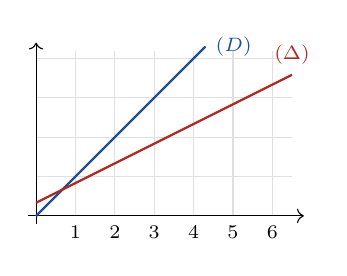
\begin{tikzpicture}[scale=0.5,font=\scriptsize]
\draw[gray!25] (0,0) grid (6.5,4.2);
\draw[->] (-0.2,0)--(6.8,0); \draw[->] (0,-0.2)--(0,4.4);
\draw[cDef,thick] (0,0)--(4.3,4.3) node[right]{$(D)$};
\draw[cThm,thick] (0,0.333)--(6.5,3.583) node[above]{$(\Delta)$};
\foreach \x in {1,...,6} \node[below] at (\x,0){$\x$};
\end{tikzpicture}
\end{LTR}}
\begin{enumerate}
\item
\begin{sq}
\qa مثّل على محور الفواصل الحدود $u_0$ ، $u_1$ ، $u_2$ ، $u_3$ و $u_4$ دون حسابها ، مبرزاً خطوط الإنشاء.
\qb عيّن إحداثيي نقطة تقاطع $(\Delta)$ و $(D)$.
\qc أعط تخميناً حول اتجاه تغير $\Un$.
\end{sq}
\item نعتبر المتتالية $(v_n)$ المعرّفة من أجل كل $n$ بـ: $v_n=u_n-\dfrac23$.
\begin{sq}
\qa بيّن أن $(v_n)$ هندسية يطلب تحديد أساسها وحدها الأول.
\qb اكتب $v_n$ ثم $u_n$ بدلالة $n$ ، واستنتج $\limn u_n$.
\qc احسب بدلالة $n$ المجموع $S_n=v_0+v_1+\cdots+v_n$ ، واستنتج $S'_n=u_0+u_1+\cdots+u_n$.
\end{sq}
\item
\begin{sq}
\qa باستعمال عبارة $u_n$ بدلالة $n$ ، بيّن أنه من أجل كل عدد طبيعي $n$: \ $u_n>\dfrac23$.
\qb احسب $u_{n+1}-u_n$ بدلالة $n$ ، ثم ادرس اتجاه تغير المتتالية $\Un$ (قارن مع التخمين).
\end{sq}
\end{enumerate}
\end{tamrin}
\begin{hal}
\RL{0.48}{%
\textbf{1.}
\begin{sq}
\qa الرسم مقابل: من $u_0=6$ نصعد إلى $(\Delta)$ ثم نتجه أفقياً إلى $(D)$ وننزل ، وهكذا.
\qb $x=\dfrac12x+\dfrac13\iff\dfrac12x=\dfrac13\iff x=\dfrac23$: \ نقطة التقاطع \bx{\Big(\dfrac23;\dfrac23\Big)}.
\qc يبدو أن $\Un$ \textbf{متناقصة} وتقترب من $\dfrac23$.
\end{sq}}{0.49}{%
\begin{LTR}\centering
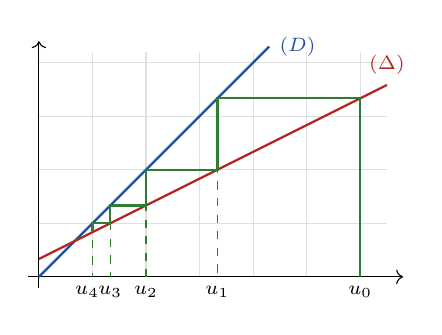
\begin{tikzpicture}[scale=0.68,font=\scriptsize]
\draw[gray!25] (0,0) grid (6.5,4.2);
\draw[->] (-0.2,0)--(6.8,0); \draw[->] (0,-0.2)--(0,4.4);
\draw[cDef,thick] (0,0)--(4.3,4.3) node[right]{$(D)$};
\draw[cThm,thick] (0,0.333)--(6.5,3.583) node[above]{$(\Delta)$};
\draw[cRem,thick] (6,0)--(6,3.333)--(3.333,3.333)--(3.333,2)--(2,2)--(2,1.333)--(1.333,1.333)--(1.333,1)--(1,1)--(1,0.833);
\draw[cRem,dashed] (3.333,3.333)--(3.333,0) (2,2)--(2,0) (1.333,1.333)--(1.333,0) (1,1)--(1,0);
\foreach \x/\n in {6/u_0,3.333/u_1,2/u_2,1.333/u_3,0.9/u_4} \node[below] at (\x,0){$\n$};
\end{tikzpicture}
\end{LTR}}
\QQ{2}
\begin{sq}
\qa $v_{n+1}=u_{n+1}-\dfrac23=\dfrac12u_n+\dfrac13-\dfrac23=\dfrac12u_n-\dfrac13=\dfrac12\Big(u_n-\dfrac23\Big)=\dfrac12v_n$.\par
$(v_n)$ هندسية أساسها \bx{q=\dfrac12} وحدها الأول $v_0=6-\dfrac23=\bx{\dfrac{16}{3}}$.
\qb $v_n=\dfrac{16}{3}\Big(\dfrac12\Big)^n$ \ و \ \bx{u_n=\dfrac23+\dfrac{16}{3}\Big(\dfrac12\Big)^n}. \ (تحقق: $u_1=\dfrac23+\dfrac83=\dfrac{10}3$ \ok.)\par
$0<\dfrac12<1$ ، إذن $\limn\Big(\dfrac12\Big)^n=0$ و $\limn u_n=\bx{\dfrac23}$.
\qc $S_n=v_0\,\dfrac{1-q^{n+1}}{1-q}=\dfrac{16}3\times\dfrac{1-\big(\frac12\big)^{n+1}}{\frac12}=\bx{\dfrac{32}{3}\Big(1-\Big(\dfrac12\Big)^{n+1}\Big)}$.\par
$u_k=v_k+\dfrac23$ ، و عدد الحدود $n+1$: \ $S'_n=S_n+\dfrac23(n+1)=\bx{\dfrac{32}{3}\Big(1-\Big(\dfrac12\Big)^{n+1}\Big)+\dfrac{2(n+1)}{3}}$.
\end{sq}
\QQ{3}
\begin{sq}
\qa $u_n-\dfrac23=v_n=\dfrac{16}{3}\Big(\dfrac12\Big)^n$ ، و $\Big(\dfrac12\Big)^n>0$ ، إذن $u_n-\dfrac23>0$ ، أي من أجل كل $n\in\N$: \bx{u_n>\dfrac23}.
\qb $u_{n+1}-u_n=\dfrac{16}{3}\Big(\dfrac12\Big)^{n+1}-\dfrac{16}{3}\Big(\dfrac12\Big)^n=\dfrac{16}{3}\Big(\dfrac12\Big)^n\Big(\dfrac12-1\Big)=\bx{-\dfrac83\Big(\dfrac12\Big)^n}<0$.\par
$\Un$ \textbf{متناقصة تماماً} ، وهذا يؤكد التخمين. \ (تحقق: $u_1-u_0=\dfrac{10}3-6=-\dfrac83$ \ok.)
\end{sq}
\begin{molahada}[تصحيح]
في الشكل الأصلي كان اسما المستقيمين متبادلين: المستقيم الذي يمر بالمبدأ هو $(D):y=x$ ، والآخر هو $(\Delta):y=\dfrac12x+\dfrac13$ (يقطع محور التراتيب في $\dfrac13$).
\end{molahada}
\end{hal}

% =====================================================================
\section{المتتاليات الحسابية}
% ------------------------------------------------- 4
\begin{tamrin}{متتالية حسابية ومجموع حدودها}
\begin{enumerate}
\item $\Un$ المتتالية المعرّفة على $\N$ بـ: $u_n=2n+5$.
\begin{sq}
\qa احسب $u_0$ ، $u_1$ و $u_2$.
\qb بيّن أن $\Un$ حسابية يطلب تعيين أساسها ، ثم استنتج اتجاه تغيرها.
\qc بيّن أن العدد $2025$ حد من حدود $\Un$ ، ثم استنتج رتبته.
\qd تحقق أن $u_0+u_1+\cdots+u_{1010}=1026165$ ، ثم احسب بدلالة $n$ المجموع $S_n=u_0+u_1+\cdots+u_n$.
\end{sq}
\item $(v_n)$ متتالية حسابية معرّفة على $\N$ بحدها الأول $v_0$ وأساسها $r$ ، حيث $v_3=13$ و $v_{10}=48$.
\begin{sq}
\qa عيّن $r$ و $v_0$.
\qb اكتب $v_n$ بدلالة $n$.
\end{sq}
\end{enumerate}
\end{tamrin}
\begin{hal}
\textbf{1.}
\begin{sq}
\qa $u_0=5$ ، $u_1=7$ ، $u_2=9$.
\qb $u_{n+1}-u_n=2(n+1)+5-2n-5=2$: \ $\Un$ حسابية أساسها \bx{r=2} ، وبما أن $r>0$ فهي \textbf{متزايدة تماماً}.
\qc $u_n=2025\iff2n+5=2025\iff n=1010\in\N$: \ $2025=u_{1010}$ ، ورتبته \bx{1011} (لأن الحد الأول $u_0$).
\qd عدد الحدود $1011$: \ $1011\times\dfrac{u_0+u_{1010}}{2}=1011\times\dfrac{5+2025}{2}=1011\times1015=1026165$ \ok.\par
$S_n=(n+1)\dfrac{5+(2n+5)}{2}=(n+1)\dfrac{2n+10}{2}=\bx{(n+1)(n+5)}$.
\end{sq}
\QQ{2}
\begin{sq}
\qa $v_{10}=v_3+(10-3)r$ ، أي $48=13+7r$ ، ومنه \bx{r=5}. \quad $v_3=v_0+3r$ ، أي $13=v_0+15$ ، ومنه \bx{v_0=-2}.
\qb \bx{v_n=-2+5n}. \ (تحقق: $v_{10}=48$ \ok.)
\end{sq}
\end{hal}

% ------------------------------------------------- 5
\begin{tamrin}{الوسط الحسابي والمجاميع}
\begin{enumerate}
\item عيّن ثلاثة أعداد هي حدود متتابعة من متتالية حسابية ، مجموعها $15$ وجداؤها $80$.
\item عيّن العدد الحقيقي $x$ حتى تكون الأعداد $x-1$ ، $2x+1$ و $4x-1$ بهذا الترتيب حدوداً متتابعة من متتالية حسابية.
\item احسب المجاميع:
\begin{sq}
\qa $A=1+2+3+\cdots+1000$
\qb $B=1+\dfrac43+\dfrac53+2+\dfrac73+\cdots+11$
\qc $C=1+3+5+\cdots+99$
\end{sq}
\end{enumerate}
\end{tamrin}
\begin{hal}
\textbf{1.} نكتبها $a-r$ ، $a$ ، $a+r$. \ المجموع: $3a=15$ ، أي $a=5$. \ الجداء: $(5-r)\times5\times(5+r)=80$ ، أي $25-r^2=16$ ، ومنه $r=3$ أو $r=-3$.\par
الأعداد هي: \bx{2\ ;\ 5\ ;\ 8} (أو $8$ ، $5$ ، $2$).
\QQ{2} الشرط: $(x-1)+(4x-1)=2(2x+1)\iff5x-2=4x+2\iff\bx{x=4}$. \ الأعداد: $3$ ، $9$ ، $15$ ($r=6$) \ok.
\QQ{3}
\begin{sq}
\qa $A=1000\times\dfrac{1+1000}{2}=\bx{500500}$.
\qb حدود حسابية أساسها $\dfrac13$ ، من $1$ إلى $11$: عدد الحدود $\dfrac{11-1}{1/3}+1=31$ ، و $B=31\times\dfrac{1+11}{2}=\bx{186}$.
\qc أعداد فردية: $99=1+2(n-1)$ يعطي $n=50$ حداً ، و $C=50\times\dfrac{1+99}{2}=\bx{2500}$.
\end{sq}
\end{hal}

% ------------------------------------------------- 6
\begin{tamrin}{متتالية تراجعية ومتتالية حسابية مساعدة}
$\Un$ متتالية عددية معرّفة على $\N$ بـ: $u_0=0$ و $u_{n+1}=\dfrac{u_n-1}{u_n+3}$.
\begin{enumerate}
\item بيّن أنه من أجل كل عدد طبيعي $n$: \ $u_{n+1}=1-\dfrac{4}{u_n+3}$.
\item احسب الحدود الخمسة الأولى للمتتالية $\Un$.
\item ادرس اتجاه تغير المتتالية $\Un$ علماً أن: $-1\le u_n\le0$.
\item نعتبر المتتالية $(v_n)$ المعرّفة على $\N$ بـ: $v_n=\dfrac{1}{u_n+1}$.
\begin{sq}
\qa بيّن أن $(v_n)$ متتالية حسابية يطلب تعيين أساسها وحدها الأول.
\qb اكتب عبارة $v_n$ بدلالة $n$ ، ثم استنتج عبارة $u_n$ بدلالة $n$.
\end{sq}
\end{enumerate}
\end{tamrin}
\begin{hal}
\textbf{1.} $1-\dfrac{4}{u_n+3}=\dfrac{u_n+3-4}{u_n+3}=\dfrac{u_n-1}{u_n+3}=u_{n+1}$ \ok.
\QQ{2} $u_0=0$ ، $u_1=-\dfrac13$ ، $u_2=\dfrac{-\frac43}{\frac83}=-\dfrac12$ ، $u_3=\dfrac{-\frac32}{\frac52}=-\dfrac35$ ، $u_4=\dfrac{-\frac85}{\frac{12}5}=-\dfrac23$.
\QQ{3} $u_{n+1}-u_n=\dfrac{u_n-1-u_n(u_n+3)}{u_n+3}=\dfrac{-u_n^2-2u_n-1}{u_n+3}=\dfrac{-(u_n+1)^2}{u_n+3}$.\par
$-1\le u_n$ ، إذن $u_n+3\ge2>0$ ، و $-(u_n+1)^2\le0$: \ $u_{n+1}-u_n\le0$ ، فـ $\Un$ \textbf{متناقصة}.
\QQ{4}
\begin{sq}
\qa $u_{n+1}+1=\dfrac{u_n-1+u_n+3}{u_n+3}=\dfrac{2(u_n+1)}{u_n+3}$ ، إذن:
\[v_{n+1}=\frac{u_n+3}{2(u_n+1)}=\frac{(u_n+1)+2}{2(u_n+1)}=\frac12+\frac{1}{u_n+1}=v_n+\frac12.\]
$(v_n)$ حسابية أساسها \bx{r=\dfrac12} وحدها الأول $v_0=\dfrac1{0+1}=\bx{1}$.
\qb $v_n=1+\dfrac n2=\bx{\dfrac{n+2}{2}}$. \ ومن $v_n=\dfrac1{u_n+1}$: $u_n=\dfrac1{v_n}-1=\dfrac{2}{n+2}-1=\bx{\dfrac{-n}{n+2}}$.\par
تحقق: $u_4=-\dfrac46=-\dfrac23$ \ok. \ (ونلاحظ $\limn u_n=-1$.)
\end{sq}
\end{hal}

% =====================================================================
\section{المتتاليات الهندسية}
% ------------------------------------------------- 7
\begin{tamrin}{متتالية هندسية ومجموع حدودها}
\begin{enumerate}
\item $(V_n)$ متتالية هندسية معرّفة على $\N$ بـ: $V_n=5\times3^n$.
\begin{sq}
\qa احسب الحدود $V_0$ ، $V_1$ ، $V_2$ و $V_3$.
\qb تحقق أن $(V_n)$ هندسية أساسها $q=3$ وحدها الأول $V_0=5$.
\qc احسب المجموع $S_n=V_0+V_1+\cdots+V_n$.
\end{sq}
\item $(w_n)$ معرّفة على $\N$ بـ: $w_n=\dfrac{3}{2^n}$. \ بيّن أن $(w_n)$ هندسية يطلب تعيين أساسها وحدها الأول ، ثم ادرس اتجاه تغيرها.
\item $(t_n)$ هندسية حدها الأول $t_0=2$ وأساسها $q=3$. \ احسب بدلالة $n$ المجموع $t_0+t_1+\cdots+t_n$.
\end{enumerate}
\end{tamrin}
\begin{hal}
\textbf{1.}
\begin{sq}
\qa $V_0=5$ ، $V_1=15$ ، $V_2=45$ ، $V_3=135$.
\qb $V_{n+1}=5\times3^{n+1}=3\times\big(5\times3^n\big)=3V_n$: \ هندسية أساسها $q=3$ و $V_0=5\times3^0=5$ \ok.
\qc $S_n=V_0\,\dfrac{1-q^{n+1}}{1-q}=5\times\dfrac{1-3^{n+1}}{1-3}=\bx{\dfrac52\big(3^{n+1}-1\big)}$. \ (تحقق $n=1$: $\dfrac52\times8=20=5+15$ \ok.)
\end{sq}
\QQ{2} $w_{n+1}=\dfrac{3}{2^{n+1}}=\dfrac{3}{2^n\times2}=\dfrac12\,w_n$: هندسية أساسها \bx{q=\dfrac12} وحدها الأول $w_0=\bx{3}$.\par
$w_0>0$ و $0<q<1$ ، إذن $(w_n)$ \textbf{متناقصة تماماً}.
\QQ{3} $t_0+\cdots+t_n=2\times\dfrac{1-3^{n+1}}{1-3}=\bx{3^{n+1}-1}$.
\end{hal}

% ------------------------------------------------- 8
\begin{tamrin}{متتالية تراجعية من الشكل $u_{n+1}=au_n+b$}
نعتبر المتتالية $\Un$ المعرّفة على $\N$ بـ: $u_0=\alpha$ و $u_{n+1}=\dfrac23u_n+1$.
\begin{enumerate}
\item عيّن قيمة $\alpha$ حتى تكون المتتالية $\Un$ ثابتة.
\item نضع $u_0=6$.
\begin{sq}
\qa احسب الحدود $u_1$ ، $u_2$ و $u_3$ ، ثم ضع تخميناً حول اتجاه تغير $\Un$.
\qb بفرض أنه من أجل كل عدد طبيعي $n$: $u_n>3$ ، ادرس اتجاه تغير $\Un$.
\end{sq}
\item نعتبر المتتالية $(v_n)$ حيث: $v_n=u_n-3$.
\begin{sq}
\qa بيّن أن $(v_n)$ هندسية أساسها $q=\dfrac23$ يطلب تعيين حدها الأول $v_0$.
\qb اكتب $v_n$ بدلالة $n$ ، ثم استنتج $u_n$ بدلالة $n$.
\qc احسب المجموعين $S_n=v_0+v_1+\cdots+v_n$ و $S'_n=u_0+u_1+\cdots+u_n$.
\end{sq}
\end{enumerate}
\end{tamrin}
\begin{hal}
\textbf{1.} $\Un$ ثابتة إذا كان $u_1=u_0$ ، أي $\dfrac23\alpha+1=\alpha\iff\dfrac13\alpha=1\iff\bx{\alpha=3}$. \ (عندئذ كل الحدود تساوي $3$.)
\QQ{2}
\begin{sq}
\qa $u_1=4+1=5$ ، $u_2=\dfrac{10}3+1=\dfrac{13}3$ ، $u_3=\dfrac{26}9+1=\dfrac{35}9$. \ \textbf{تخمين:} $\Un$ متناقصة.
\qb $u_{n+1}-u_n=-\dfrac13u_n+1=-\dfrac13\big(u_n-3\big)<0$ لأن $u_n>3$: \ $\Un$ \textbf{متناقصة تماماً}.
\end{sq}
\QQ{3}
\begin{sq}
\qa $v_{n+1}=u_{n+1}-3=\dfrac23u_n-2=\dfrac23\big(u_n-3\big)=\dfrac23v_n$: هندسية أساسها $\dfrac23$ ، و $v_0=6-3=\bx{3}$.
\qb $v_n=\bx{3\Big(\dfrac23\Big)^n}$ \ و \ $u_n=v_n+3=\bx{3+3\Big(\dfrac23\Big)^n}$. \ (تحقق: $u_2=3+\dfrac43=\dfrac{13}3$ \ok.)
\qc $S_n=3\times\dfrac{1-\big(\frac23\big)^{n+1}}{1-\frac23}=\bx{9\Big(1-\Big(\dfrac23\Big)^{n+1}\Big)}$ \quad ؛ \quad $S'_n=S_n+3(n+1)=\bx{9\Big(1-\Big(\dfrac23\Big)^{n+1}\Big)+3n+3}$.
\end{sq}
\end{hal}

% ------------------------------------------------- 9
\begin{tamrin}{متتالية هندسية مساعدة ونهاية}
لتكن $\Un$ متتالية عددية معرّفة على $\N$ بحدها الأول $u_0=1$ ، ومن أجل كل $n$: $u_{n+1}=\dfrac13u_n+\dfrac13$. \ ولتكن $(v_n)$ المعرّفة بـ: $v_n=u_n-\dfrac12$.
\begin{enumerate}
\item احسب الحدود $u_1$ ، $u_2$ ، $u_3$ ، ثم ضع تخميناً حول اتجاه تغير $\Un$.
\item بيّن أن $(v_n)$ هندسية يطلب تعيين أساسها وحدها الأول $v_0$.
\item اكتب عبارة $v_n$ بدلالة $n$ ، ثم استنتج $u_n$ بدلالة $n$.
\item ادرس اتجاه تغير $(v_n)$ ، ثم استنتج اتجاه تغير $\Un$ ، واحسب $\limn u_n$.
\item احسب بدلالة $n$ المجموع $S_n=v_0+v_1+\cdots+v_n$ ، ثم استنتج $S'_n=u_0+u_1+\cdots+u_n$.
\end{enumerate}
\end{tamrin}
\begin{hal}
\textbf{1.} $u_1=\dfrac13+\dfrac13=\dfrac23$ ، $u_2=\dfrac29+\dfrac13=\dfrac59$ ، $u_3=\dfrac5{27}+\dfrac13=\dfrac{14}{27}$. \ \textbf{تخمين:} $\Un$ متناقصة.
\QQ{2} $v_{n+1}=\dfrac13u_n+\dfrac13-\dfrac12=\dfrac13u_n-\dfrac16=\dfrac13\Big(u_n-\dfrac12\Big)=\dfrac13v_n$: هندسية أساسها \bx{q=\dfrac13} و $v_0=1-\dfrac12=\bx{\dfrac12}$.
\QQ{3} $v_n=\bx{\dfrac12\Big(\dfrac13\Big)^n}$ \ و \ $u_n=\bx{\dfrac12+\dfrac12\Big(\dfrac13\Big)^n}$. \ (تحقق: $u_1=\dfrac12+\dfrac16=\dfrac23$ \ok.)
\QQ{4} $v_0>0$ و $0<q<1$: $(v_n)$ متناقصة تماماً ، و $u_n=v_n+\dfrac12$ ، فـ $u_{n+1}-u_n=v_{n+1}-v_n<0$: \ $\Un$ \textbf{متناقصة تماماً}.\par
$\limn\Big(\dfrac13\Big)^n=0$ ، إذن $\limn u_n=\bx{\dfrac12}$.
\QQ{5} $S_n=\dfrac12\times\dfrac{1-\big(\frac13\big)^{n+1}}{1-\frac13}=\bx{\dfrac34\Big(1-\Big(\dfrac13\Big)^{n+1}\Big)}$ \quad ؛ \quad $S'_n=S_n+\dfrac{n+1}{2}=\bx{\dfrac34\Big(1-\Big(\dfrac13\Big)^{n+1}\Big)+\dfrac{n+1}2}$.
\end{hal}

% ------------------------------------------------- 10
\begin{tamrin}{الوسط الهندسي}
\begin{enumerate}
\item عيّن ثلاثة أعداد هي حدود متتابعة من متتالية هندسية ، جداؤها $64$ ومجموعها $21$.
\item عيّن العدد الحقيقي الموجب $x$ حتى تكون الأعداد $x$ ، $x+2$ و $4x-1$ بهذا الترتيب حدوداً متتابعة من متتالية هندسية.
\end{enumerate}
\end{tamrin}
\begin{hal}
\textbf{1.} نكتبها $\dfrac aq$ ، $a$ ، $aq$. \ الجداء: $a^3=64$ ، إذن $a=4$. \ المجموع: $\dfrac4q+4+4q=21$ ، وبالضرب في $q$: $4q^2-17q+4=0$.\par
$\Delta=289-64=225$: \ $q=\dfrac{17+15}{8}=4$ أو $q=\dfrac{17-15}8=\dfrac14$. \ الأعداد: \bx{1\ ;\ 4\ ;\ 16} (أو $16$ ، $4$ ، $1$).
\QQ{2} الشرط: $x(4x-1)=(x+2)^2\iff4x^2-x=x^2+4x+4\iff3x^2-5x-4=0$.\par
$\Delta=25+48=73$: \ $x=\dfrac{5+\sqrt{73}}{6}\approx2{,}26$ (الحل الموجب) ، و $x=\dfrac{5-\sqrt{73}}6<0$ مرفوض: \ \bx{x=\dfrac{5+\sqrt{73}}{6}}.
\end{hal}

% =====================================================================
\section{نهاية متتالية}
% ------------------------------------------------- 11
\begin{tamrin}{حساب نهايات}
\begin{enumerate}
\item احسب نهاية كل متتالية مما يلي (عند $+\infty$):
\begin{sq}
\qa $a_n=\dfrac{2n+1}{n+3}$
\qb $b_n=\dfrac{n^2+1}{2n^2-n}$ \ ($n\ge1$)
\qc $c_n=-n^2+3n$
\qd $d_n=\Big(\dfrac{-3}{4}\Big)^n$
\qe $e_n=-2\times6^n$
\end{sq}
\item هل المتتالية $u_n=2+(-1)^n$ متقاربة؟ \ وهل $f_n=5\Big(\dfrac13\Big)^n+2$ متقاربة؟
\item $\Un$ متتالية حسابية حدها الأول $u_0=7$ وأساسها $3$. \ أوجد $u_n$ ، ثم احسب $S=u_0+u_1+\cdots+u_{200}$ ، وعيّن $\limn u_n$.
\end{enumerate}
\end{tamrin}
\begin{hal}
\textbf{1.}
\begin{sq}
\qa $\limn a_n=\limn\dfrac{2n}{n}=\bx{2}$.
\qb $\limn b_n=\limn\dfrac{n^2}{2n^2}=\bx{\dfrac12}$.
\qc $c_n=n^2\Big(-1+\dfrac3n\Big)$ ، و $\limn c_n=\bx{-\infty}$.
\qd $-1<-\dfrac34<1$ ، إذن $\limn d_n=\bx{0}$.
\qe $6>1$ ، $\limn6^n=+\infty$ ، و $-2<0$: \ $\limn e_n=\bx{-\infty}$.
\end{sq}
\QQ{2} $u_n$ تساوي $3$ إذا كان $n$ زوجياً و $1$ إذا كان فردياً: لا تقترب من عدد واحد ، فهي \textbf{متباعدة} (النهاية غير موجودة).\par
$0<\dfrac13<1$: $\limn f_n=0+2=2$ ، فـ $(f_n)$ \textbf{متقاربة} نحو $2$.
\QQ{3} $u_n=7+3n$. \ $u_{200}=607$ ، و $S=201\times\dfrac{7+607}{2}=201\times307=\bx{61707}$. \quad $r=3>0$: \ $\limn u_n=\bx{+\infty}$.
\end{hal}

% =====================================================================
\section{مسائل شاملة}
% ------------------------------------------------- 12
\begin{tamrin}{متتالية هوموغرافية}
في الشكل ، $(C_f)$ هو تمثيل الدالة $f$ المعرّفة على $[0;5]$ بـ: $f(x)=\dfrac{4x-1}{x+2}$ ، و $(d)$ المستقيم ذو المعادلة $y=x$.\par
$\Un$ المتتالية المعرّفة بـ: $u_0=3$ ، ومن أجل كل $n$: $u_{n+1}=f(u_n)$.
\begin{enumerate}
\item مثّل على محور الفواصل الحدود $u_0$ ، $u_1$ ، $u_2$ و $u_3$ دون حسابها ، ثم أعط تخميناً حول اتجاه تغير $\Un$.
\item ادرس اتجاه تغير $\Un$ علماً أن $u_n>1$ من أجل كل $n$.
\item من أجل كل $n$ نضع: $v_n=\dfrac{1}{u_n-1}$.
\begin{sq}
\qa احسب $v_0$ ، ثم برهن أن $(v_n)$ حسابية أساسها $\dfrac13$.
\qb اكتب $v_n$ بدلالة $n$ ، ثم استنتج $u_n$ بدلالة $n$.
\qc احسب المجموع $S_n=v_0+v_1+\cdots+v_n$.
\end{sq}
\end{enumerate}
\end{tamrin}
\begin{hal}
\RL{0.48}{%
\textbf{1.} الرسم مقابل: $u_0=3$ ، $u_1=2{,}2$ ، $u_2\approx1{,}86$ ، $u_3\approx1{,}67$.\par
\textbf{تخمين:} $\Un$ متناقصة وتقترب من $1$ (فاصلة نقطة تقاطع $(C_f)$ و $(d)$ ، حيث $(C_f)$ مماس لـ $(d)$).
\QQ{2} $u_{n+1}-u_n=\dfrac{4u_n-1-u_n(u_n+2)}{u_n+2}=\dfrac{-u_n^2+2u_n-1}{u_n+2}$\par
$=\dfrac{-(u_n-1)^2}{u_n+2}<0$ \ (لأن $u_n>1$).\par
$\Un$ \textbf{متناقصة تماماً}.}{0.49}{%
\begin{LTR}\centering
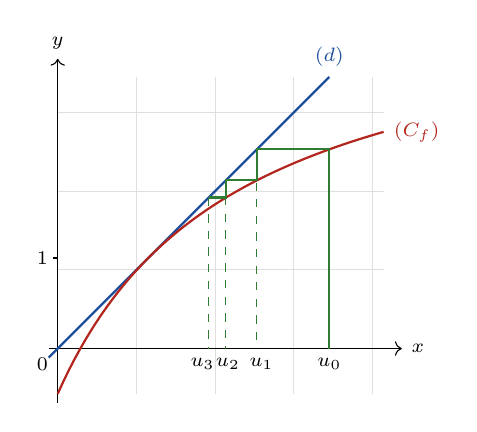
\begin{tikzpicture}[x=1.15cm,y=1.15cm,font=\scriptsize]
\draw[gray!25] (0,-0.5) grid (3.6,3);
\draw[->] (-0.1,0)--(3.8,0) node[right]{$x$}; \draw[->] (0,-0.6)--(0,3.2) node[above]{$y$};
\draw[cDef,thick] (-0.1,-0.1)--(3,3) node[above]{$(d)$};
\draw[cThm,thick,domain=0:3.6,samples=60] plot (\x,{(4*\x-1)/(\x+2)}) node[right]{$(C_f)$};
\draw[cRem,thick] (3,0)--(3,2.2)--(2.2,2.2)--(2.2,1.857)--(1.857,1.857)--(1.857,1.667)--(1.667,1.667);
\draw[cRem,dashed] (2.2,2.2)--(2.2,0) (1.857,1.857)--(1.857,0) (1.667,1.667)--(1.667,0);
\foreach \x/\n in {3/u_0,2.25/u_1,1.88/u_2,1.6/u_3} \node[below] at (\x,0){$\n$};
\node[below left] at (0,0){$0$}; \node[left] at (0,1){$1$}; \draw (0,1)--(-0.05,1);
\end{tikzpicture}
\end{LTR}}
\QQ{3}
\begin{sq}
\qa $v_0=\dfrac1{3-1}=\bx{\dfrac12}$. \quad $u_{n+1}-1=\dfrac{4u_n-1-u_n-2}{u_n+2}=\dfrac{3(u_n-1)}{u_n+2}$ ، إذن:
\[v_{n+1}=\frac{u_n+2}{3(u_n-1)}=\frac{(u_n-1)+3}{3(u_n-1)}=\frac13+\frac1{u_n-1}=v_n+\frac13.\]
$(v_n)$ حسابية أساسها $\dfrac13$.
\qb $v_n=\dfrac12+\dfrac n3=\bx{\dfrac{2n+3}{6}}$ \ و \ $u_n=1+\dfrac1{v_n}=1+\dfrac{6}{2n+3}=\bx{\dfrac{2n+9}{2n+3}}$. \ (تحقق: $u_1=\dfrac{11}5$ \ok.)
\qc $S_n=(n+1)\dfrac{v_0+v_n}{2}=(n+1)\dfrac{\frac12+\frac12+\frac n3}{2}=\bx{\dfrac{(n+1)(n+3)}{6}}$.
\end{sq}
\end{hal}

% ------------------------------------------------- 13
\begin{tamrin}{متتالية تراجعية ومتتالية حسابية: مجموع معطى}
$\Un$ متتالية معرّفة بحدها الأول $u_0=2$ وبالعلاقة: $u_{n+1}=\dfrac{u_n}{2u_n+1}$. \ $(C_f)$ هو تمثيل الدالة $f(x)=\dfrac{x}{2x+1}$ على $\Big]-\dfrac12;+\infty\Big[$ ، و $(\Delta):y=x$.
\begin{enumerate}
\item
\begin{sq}
\qa مثّل على محور الفواصل الحدود $u_0$ ، $u_1$ و $u_2$ دون حسابها مبرزاً خطوط الرسم.
\qb ضع تخميناً حول اتجاه تغير $\Un$.
\qc إذا علمت أنه من أجل كل $n$: $u_n>0$ ، بيّن أن $\Un$ متناقصة تماماً.
\end{sq}
\item نعتبر المتتالية $(v_n)$ المعرّفة على $\N$ بـ: $v_n=\dfrac{1-u_n}{u_n}$ \ (حيث $u_n\ne0$).
\begin{sq}
\qa أثبت أن $(v_n)$ حسابية أساسها $2$ يطلب تعيين حدها الأول.
\qb اكتب $v_n$ بدلالة $n$ ، ثم استنتج أن $u_n=\dfrac{2}{4n+1}$.
\qc احسب بدلالة $n$ المجموع $S_n=\dfrac12v_0+\dfrac12v_1+\cdots+\dfrac12v_n$ ، ثم عيّن قيمة $n$ حتى يكون $S_n=2000$.
\end{sq}
\end{enumerate}
\end{tamrin}
\begin{hal}
\RL{0.52}{%
\textbf{1.}
\begin{sq}
\qa الرسم مقابل ($u_0=2$ ، $u_1=0{,}4$ ، $u_2\approx0{,}22$).
\qb \textbf{تخمين:} $\Un$ متناقصة وتقترب من $0$.
\qc $u_{n+1}-u_n=\dfrac{u_n-u_n(2u_n+1)}{2u_n+1}=\dfrac{-2u_n^2}{2u_n+1}$.\par
بما أن $u_n>0$: البسط سالب تماماً والمقام موجب ، إذن $u_{n+1}-u_n<0$ ، و $\Un$ \textbf{متناقصة تماماً}.
\end{sq}}{0.45}{%
\begin{LTR}\centering
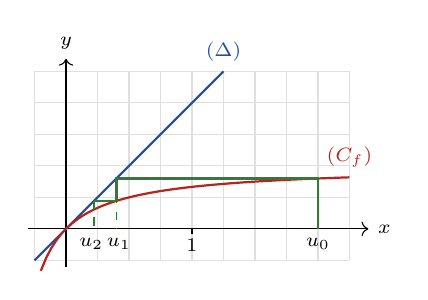
\begin{tikzpicture}[x=1.6cm,y=1.6cm,font=\scriptsize]
\draw[gray!25,step=0.25] (-0.25,-0.25) grid (2.25,1.25);
\draw[->] (-0.3,0)--(2.4,0) node[right]{$x$}; \draw[->] (0,-0.3)--(0,1.35) node[above]{$y$};
\draw[cDef,thick] (-0.25,-0.25)--(1.25,1.25) node[above]{$(\Delta)$};
\draw[cThm,thick,domain=-0.2:2.25,samples=60] plot (\x,{\x/(2*\x+1)}) node[above]{$(C_f)$};
\draw[cRem,thick] (2,0)--(2,0.4)--(0.4,0.4)--(0.4,0.222)--(0.222,0.222);
\draw[cRem,dashed] (0.4,0.4)--(0.4,0) (0.222,0.222)--(0.222,0);
\foreach \x/\n in {2/u_0,0.42/u_1,0.2/u_2} \node[below] at (\x,0){$\n$};
\node[below] at (1,0){$1$}; \draw (1,0)--(1,-0.04);
\end{tikzpicture}
\end{LTR}}
\QQ{2}
\begin{sq}
\qa $v_n=\dfrac1{u_n}-1$ ، و $\dfrac1{u_{n+1}}=\dfrac{2u_n+1}{u_n}=2+\dfrac1{u_n}$ ، إذن $v_{n+1}=\dfrac1{u_{n+1}}-1=2+\dfrac1{u_n}-1=v_n+2$.\par
$(v_n)$ حسابية أساسها $2$ وحدها الأول $v_0=\dfrac{1-2}{2}=\bx{-\dfrac12}$.
\qb $v_n=-\dfrac12+2n=\bx{\dfrac{4n-1}{2}}$. \ ومن $v_n=\dfrac1{u_n}-1$: $u_n=\dfrac1{v_n+1}=\dfrac{1}{\frac{4n+1}{2}}=\bx{\dfrac2{4n+1}}$ \ok.
\qc $S_n=\dfrac12\big(v_0+\cdots+v_n\big)=\dfrac12(n+1)\dfrac{-\frac12+\frac{4n-1}{2}}{2}=\bx{\dfrac{(n+1)(2n-1)}{4}}$.\par
$S_n=2000\iff(n+1)(2n-1)=8000\iff2n^2+n-8001=0$. \ $\Delta=1+64008=64009=253^2$:\par
$n=\dfrac{-1+253}{4}=\bx{63}$ (الحل الآخر سالب). \ تحقق: $64\times125=8000$ \ok.
\end{sq}
\end{hal}

% ------------------------------------------------- 14
\begin{tamrin}{متتاليتان متشابكتان}
نعتبر المتتاليتين $\Un$ و $(V_n)$ المعرّفتين بحديهما الأولين $U_0=2$ و $V_0=-1$ ، ومن أجل كل عدد طبيعي $n$ بالعلاقتين:
\[\begin{cases}U_{n+1}=(1+\alpha)U_n-\alpha V_n\\[2pt] V_{n+1}=(1-\alpha)U_n+\alpha V_n\end{cases}\qquad\text{\ar{حيث $\alpha$ وسيط حقيقي غير معدوم.}}\]
\begin{enumerate}
\item برهن باستعمال العلاقتين أنه إذا كانت $(U_n)$ متقاربة نحو $\ell$ فإن $(V_n)$ متقاربة كذلك نحو $\ell$.
\item نفرض أن $\alpha=\dfrac12$.
\begin{sq}
\qa بيّن أنه من أجل كل $n$: $U_n-V_n=3$ ، ثم استنتج أن $(U_n)$ حسابية يطلب تعيين أساسها.
\qb احسب بدلالة $n$ المجموع $S_n=U_0+U_1+\cdots+U_n$.
\end{sq}
\item نفرض أن $\alpha\ne\dfrac12$ ، ونعرّف المتتالية $(W_n)$ بـ: $W_n=U_n-V_n$.
\begin{sq}
\qa بيّن أن $(W_n)$ هندسية أساسها $q=2\alpha$.
\qb اكتب $W_n$ بدلالة $n$ و $\alpha$ ، ثم احسب المجموع $T_n=W_0+W_1+\cdots+W_n$.
\qc بيّن أنه من أجل كل $n\in\N$: \ $U_{n+1}-U_n=\alpha W_n$.
\qd استنتج أن: $U_n=\dfrac{3\times2^n\times\alpha^{n+1}+\alpha-2}{2\alpha-1}$.
\qe عيّن قيم $\alpha$ التي من أجلها تكون $(U_n)$ متقاربة ، ثم احسب نهايتها.
\end{sq}
\end{enumerate}
\end{tamrin}
\begin{hal}
\textbf{1.} من العلاقة الأولى: $\alpha V_n=(1+\alpha)U_n-U_{n+1}$ ، أي $V_n=\dfrac{(1+\alpha)U_n-U_{n+1}}{\alpha}$ ($\alpha\ne0$).\par
إذا كانت $\limn U_n=\ell$ فإن $\limn U_{n+1}=\ell$ ، ومنه $\limn V_n=\dfrac{(1+\alpha)\ell-\ell}{\alpha}=\dfrac{\alpha\ell}{\alpha}=\bx{\ell}$.
\QQ{2}
\begin{sq}
\qa بطرح العلاقتين: $U_{n+1}-V_{n+1}=2\alpha U_n-2\alpha V_n=2\alpha\big(U_n-V_n\big)$. \ مع $\alpha=\dfrac12$: $U_{n+1}-V_{n+1}=U_n-V_n$ ، فالفرق ثابت ويساوي $U_0-V_0=3$.\par
$U_{n+1}=\dfrac32U_n-\dfrac12V_n=U_n+\dfrac12\big(U_n-V_n\big)=U_n+\dfrac32$: \ $(U_n)$ حسابية أساسها \bx{r=\dfrac32}.
\qb $U_n=2+\dfrac32n$ ، و $S_n=(n+1)\dfrac{2+2+\frac32n}{2}=\bx{\dfrac{(n+1)(3n+8)}{4}}$.
\end{sq}
\begin{molahada}[تصحيح]
نص السؤال الأصلي يذكر أن الأساس $r=3$ ، والصحيح \bx{r=\dfrac32}: \ $U_0=2$ ، $U_1=\dfrac32\times2-\dfrac12\times(-1)=\dfrac72$ ، و $U_1-U_0=\dfrac32$.
\end{molahada}
\QQ{3}
\begin{sq}
\qa وجدنا في 2(أ): $W_{n+1}=2\alpha\,W_n$: \ $(W_n)$ هندسية أساسها $q=2\alpha$ ، وحدها الأول $W_0=3$.
\qb $W_n=\bx{3(2\alpha)^n}$. \quad $q\ne1$ (لأن $\alpha\ne\frac12$): \ $T_n=3\times\dfrac{1-(2\alpha)^{n+1}}{1-2\alpha}$.
\qc $U_{n+1}-U_n=(1+\alpha)U_n-\alpha V_n-U_n=\alpha U_n-\alpha V_n=\alpha W_n$ \ok.
\qd بجمع المساويات $U_{k+1}-U_k=\alpha W_k$ من $k=0$ إلى $n-1$ (المجموع تلسكوبي):
\[U_n-U_0=\alpha\big(W_0+\cdots+W_{n-1}\big)=3\alpha\,\frac{1-(2\alpha)^n}{1-2\alpha}.\]
$U_n=2+\dfrac{3\alpha-3\alpha(2\alpha)^n}{1-2\alpha}=\dfrac{2-4\alpha+3\alpha-3\times2^n\alpha^{n+1}}{1-2\alpha}=\dfrac{2-\alpha-3\times2^n\alpha^{n+1}}{1-2\alpha}=\bx{\dfrac{3\times2^n\times\alpha^{n+1}+\alpha-2}{2\alpha-1}}$.
\qe $2^n\alpha^{n+1}=\alpha(2\alpha)^n$: تتقارب $(U_n)$ إذا وفقط إذا تقاربت $(2\alpha)^n$ ، أي $-1<2\alpha<1$ (الحالة $2\alpha=1$ مستبعدة).\par
إذن: \bx{\alpha\in\Big]-\dfrac12;0\Big[\cup\Big]0;\dfrac12\Big[} \ ، وعندئذ $\limn(2\alpha)^n=0$ و \bx{\limn U_n=\dfrac{\alpha-2}{2\alpha-1}=\dfrac{2-\alpha}{1-2\alpha}}.
\end{sq}
\end{hal}

% =====================================================================
\section{اختيار من متعدد ، صحيح أم خطأ}
% ------------------------------------------------- 15
\begin{tamrin}{اختيار من متعدد}
لكل سؤال جواب واحد صحيح من بين الأجوبة الثلاثة ، عيّنه مع التعليل:
\begin{enumerate}
\item $\Un$ حسابية حدها الأول $u_0=2$ وأساسها $r$ ، وتحقق: $u_0+\dfrac12u_4=u_3-1$. \ قيمة $r$ هي:
\ABC{$r=-2$}{$r=\dfrac12$}{$r=2$}
\item $(v_n)$ غير ثابتة معرّفة بـ: $v_{n+1}=(\alpha+1)v_n+1$. \ تكون $(v_n)$ حسابية من أجل:
\ABC{$\alpha=0$}{$\alpha=-1$}{$\alpha=1$}
\item $\Un$ هندسية ، $u_0=3$ و $q=2$. \ الحد $u_5$ يساوي:
\ABC{$30$}{$96$}{$192$}
\item المجموع $1+2+2^2+\cdots+2^{10}$ يساوي:
\ABC{$2047$}{$2048$}{$1023$}
\item $\Un$ حسابية حيث $u_5=17$ و $u_{12}=38$. \ أساسها هو:
\ABC{$3$}{$7$}{$-3$}
\item $\limn\Big(5\Big(\dfrac23\Big)^n+1\Big)$ تساوي:
\ABC{$+\infty$}{$1$}{$6$}
\item المتتالية $u_n=(-2)^n$:
\ABC{متزايدة}{متناقصة}{ليست رتيبة}
\item عدد الحدود من $u_7$ إلى $u_{40}$ هو:
\ABC{$33$}{$34$}{$40$}
\end{enumerate}
\end{tamrin}
\begin{hal}
\textbf{1.} (جـ): $u_4=2+4r$ ، $u_3=2+3r$: \ $2+1+2r=1+3r$ ، أي $r=2$.
\QQ{2} (أ): يجب أن يكون معامل $v_n$ يساوي $1$: $\alpha+1=1$ ، أي $\alpha=0$ ، فتصبح $v_{n+1}=v_n+1$ (أساسها $1$).
\QQ{3} (ب): $u_5=3\times2^5=96$.
\QQ{4} (أ): $11$ حداً ، $1\times\dfrac{1-2^{11}}{1-2}=2^{11}-1=2047$.
\QQ{5} (أ): $38=17+7r$ ، $r=3$.
\QQ{6} (ب): $0<\dfrac23<1$ ، فـ $\Big(\dfrac23\Big)^n\to0$ والنهاية $1$.
\QQ{7} (جـ): $u_0=1$ ، $u_1=-2$ ، $u_2=4$: الإشارات تتناوب.
\QQ{8} (ب): $40-7+1=34$.
\end{hal}

% ------------------------------------------------- 16
\begin{tamrin}{صحيح أم خطأ}
أجب بصحيح أو خطأ مع التبرير:
\begin{enumerate}
\item إذا كانت المتتالية الحسابية $\Un$ متزايدة تماماً فإن أساسها أكبر تماماً من $0$.
\item $\Un$ متتالية حسابية أساسها $r=2$ ، لدينا $u_{n+1}=u_n-2$.
\item $\Un$ حسابية أساسها $r=2$ وحدها الأول $u_1=5$ ، عبارة حدها العام هي: $u_n=3+2n$.
\item $1+2+3+\cdots+999+1000=1001000$.
\item $\alpha$ عدد حقيقي غير معدوم ، و $(v_n)$ معرّفة بـ $v_0=1$ و $v_{n+1}=\dfrac1\alpha v_n$. \ قيمة $\alpha$ حتى تكون $(v_n)$ ثابتة هي $\alpha=2$.
\item $(w_n)$ حسابية أساسها $r=1$ وحدها الأول $w_1=2$. \ مجموع حدودها الـ $n$ الأولى هو $\dfrac{n(n+3)}{2}$.
\item كل متتالية هندسية أساسها $q=-2$ هي متتالية رتيبة.
\item إذا كان $u_n=f(n)$ و $f$ متزايدة على $[0;+\infty[$ فإن $\Un$ متزايدة.
\end{enumerate}
\end{tamrin}
\begin{hal}
\textbf{1.} \textbf{صحيح:} $u_{n+1}-u_n=r>0$.
\QQ{2} \textbf{خطأ:} $u_{n+1}=u_n-2$ معناه أن الأساس $r=-2$.
\QQ{3} \textbf{صحيح:} $u_n=u_1+(n-1)r=5+2n-2=3+2n$.
\QQ{4} \textbf{خطأ:} $1000\times\dfrac{1+1000}2=500500$.
\QQ{5} \textbf{خطأ:} $(v_n)$ ثابتة إذا كان $\dfrac1\alpha=1$ ، أي $\alpha=1$ (مع $\alpha=2$: $v_1=\dfrac12\ne v_0$).
\QQ{6} \textbf{صحيح:} $w_n=n+1$ ، و $w_1+\cdots+w_n=n\times\dfrac{2+(n+1)}{2}=\dfrac{n(n+3)}2$.
\QQ{7} \textbf{خطأ:} إشارات الحدود تتناوب (إذا كان $u_0\ne0$) ، فهي ليست رتيبة.
\QQ{8} \textbf{صحيح:} $n<n+1$ و $f$ متزايدة ، إذن $f(n)\le f(n+1)$.
\end{hal}

% =====================================================================
\section{تمرين نموذجي}
% ------------------------------------------------- 17
\begin{tamrin}{تمرين نموذجي: متتالية متباعدة}
$\Un$ المتتالية المعرّفة على $\N$ بـ: $u_0=3$ و $u_{n+1}=3u_n-4$.
\begin{enumerate}
\item احسب $u_1$ ، $u_2$ و $u_3$. \ هل $\Un$ حسابية؟ هل هي هندسية؟
\item نضع $v_n=u_n-2$.
\begin{sq}
\qa بيّن أن $(v_n)$ هندسية يطلب تعيين أساسها وحدها الأول.
\qb اكتب $u_n$ بدلالة $n$ ، ثم احسب $\limn u_n$.
\qc عيّن أصغر عدد طبيعي $n$ حيث $u_n>1000$.
\qd احسب بدلالة $n$ المجموع $S'_n=u_0+u_1+\cdots+u_n$.
\end{sq}
\item استنتج أنه من أجل كل $n$: $u_n>2$ ، ثم ادرس اتجاه تغير $\Un$ بإشارة $u_{n+1}-u_n$.
\end{enumerate}
\end{tamrin}
\begin{hal}
\textbf{1.} $u_1=9-4=5$ ، $u_2=15-4=11$ ، $u_3=33-4=29$.\par
$u_1-u_0=2\ne u_2-u_1=6$: \textbf{ليست حسابية}. \quad $\dfrac{u_1}{u_0}=\dfrac53\ne\dfrac{u_2}{u_1}=\dfrac{11}5$: \textbf{ليست هندسية}.
\QQ{2}
\begin{sq}
\qa $v_{n+1}=3u_n-4-2=3(u_n-2)=3v_n$: هندسية أساسها \bx{q=3} وحدها الأول $v_0=\bx{1}$.
\qb $v_n=3^n$ ، و \bx{u_n=2+3^n}. \ $3>1$ ، إذن $\limn3^n=+\infty$ و $\limn u_n=\bx{+\infty}$ ($\Un$ متباعدة).
\qc $u_n>1000\iff3^n>998$. \ $3^6=729<998$ و $3^7=2187>998$ ، و $(3^n)$ متزايدة: \ أصغر عدد هو \bx{n=7} ($u_7=2189$).
\qd $S'_n=\big(v_0+\cdots+v_n\big)+2(n+1)=\dfrac{3^{n+1}-1}{3-1}+2(n+1)=\bx{\dfrac{3^{n+1}-1}{2}+2n+2}$. \ (تحقق $n=1$: $\dfrac{9-1}{2}+4=8=u_0+u_1$ \ok.)
\end{sq}
\QQ{3} $u_n-2=3^n>0$ ، إذن من أجل كل $n\in\N$: \bx{u_n>2}.\par
$u_{n+1}-u_n=\big(2+3^{n+1}\big)-\big(2+3^n\big)=3^n(3-1)=2\times3^n>0$: \ $\Un$ \textbf{متزايدة تماماً}.
\end{hal}

\end{document}
